
\section{Introduction} 
\label{sec:introduction}
% \vspace{-1ex}
% \begin{figure}[t]
%     \centering
%     \begin{minipage}{0.45\textwidth}
%         \centering
%         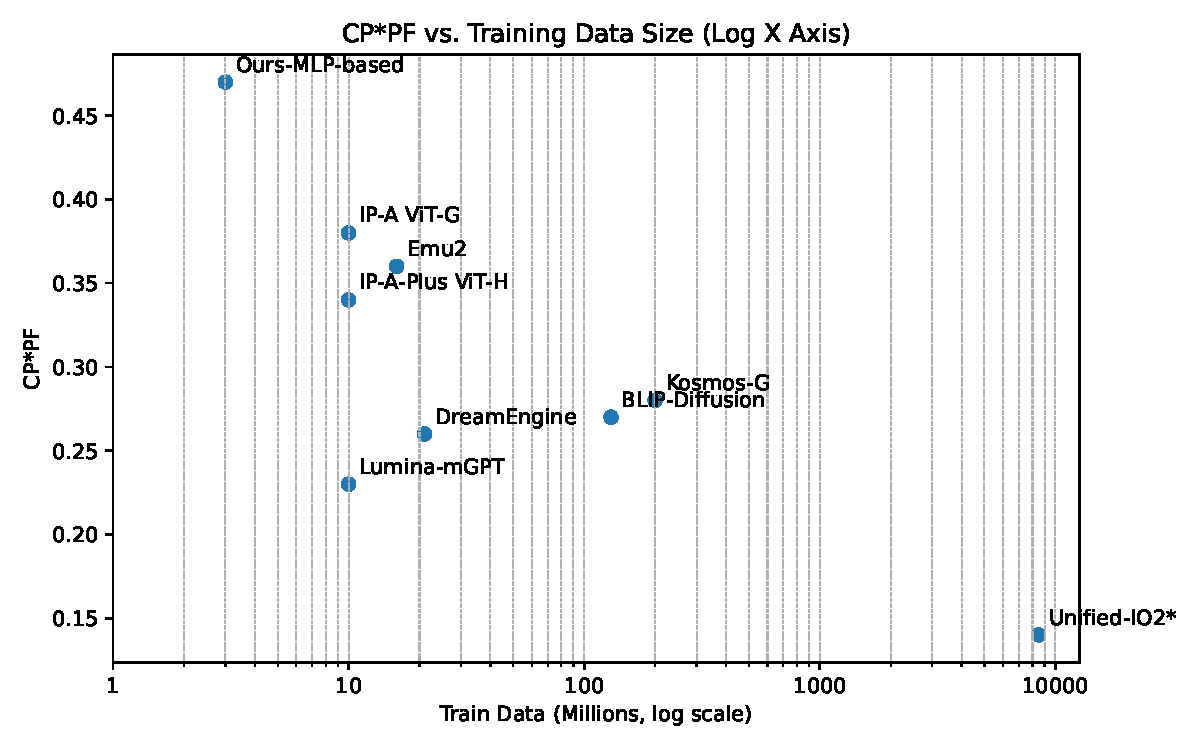
\includegraphics[width=\textwidth]{figures/data.pdf}
%         \caption{data}
%         \label{fig:data}
%     \end{minipage}
%     \hfill
%     \begin{minipage}{0.45\textwidth}
%         \centering
%         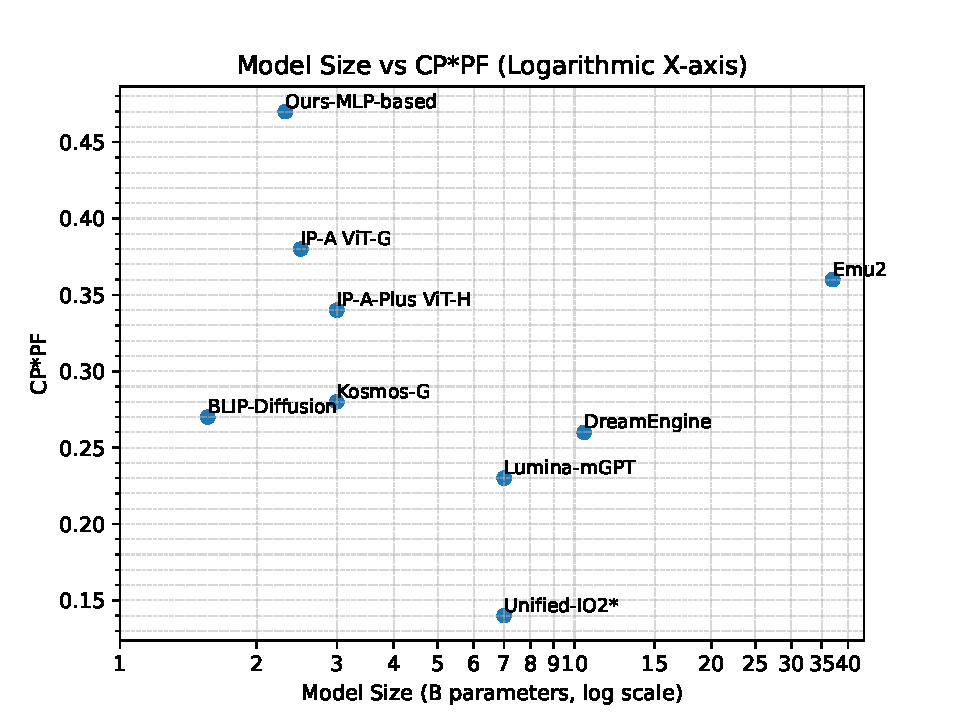
\includegraphics[width=\textwidth]{figures/size.pdf}
%         \caption{size}
%         \label{fig:size}
%     \end{minipage}
%     \caption{Caption text here}
%     \label{fig:comparison}
% \end{figure}

\begin{wrapfigure}{r}{0.50\textwidth} 
    \centering
    \vspace{-5mm}
    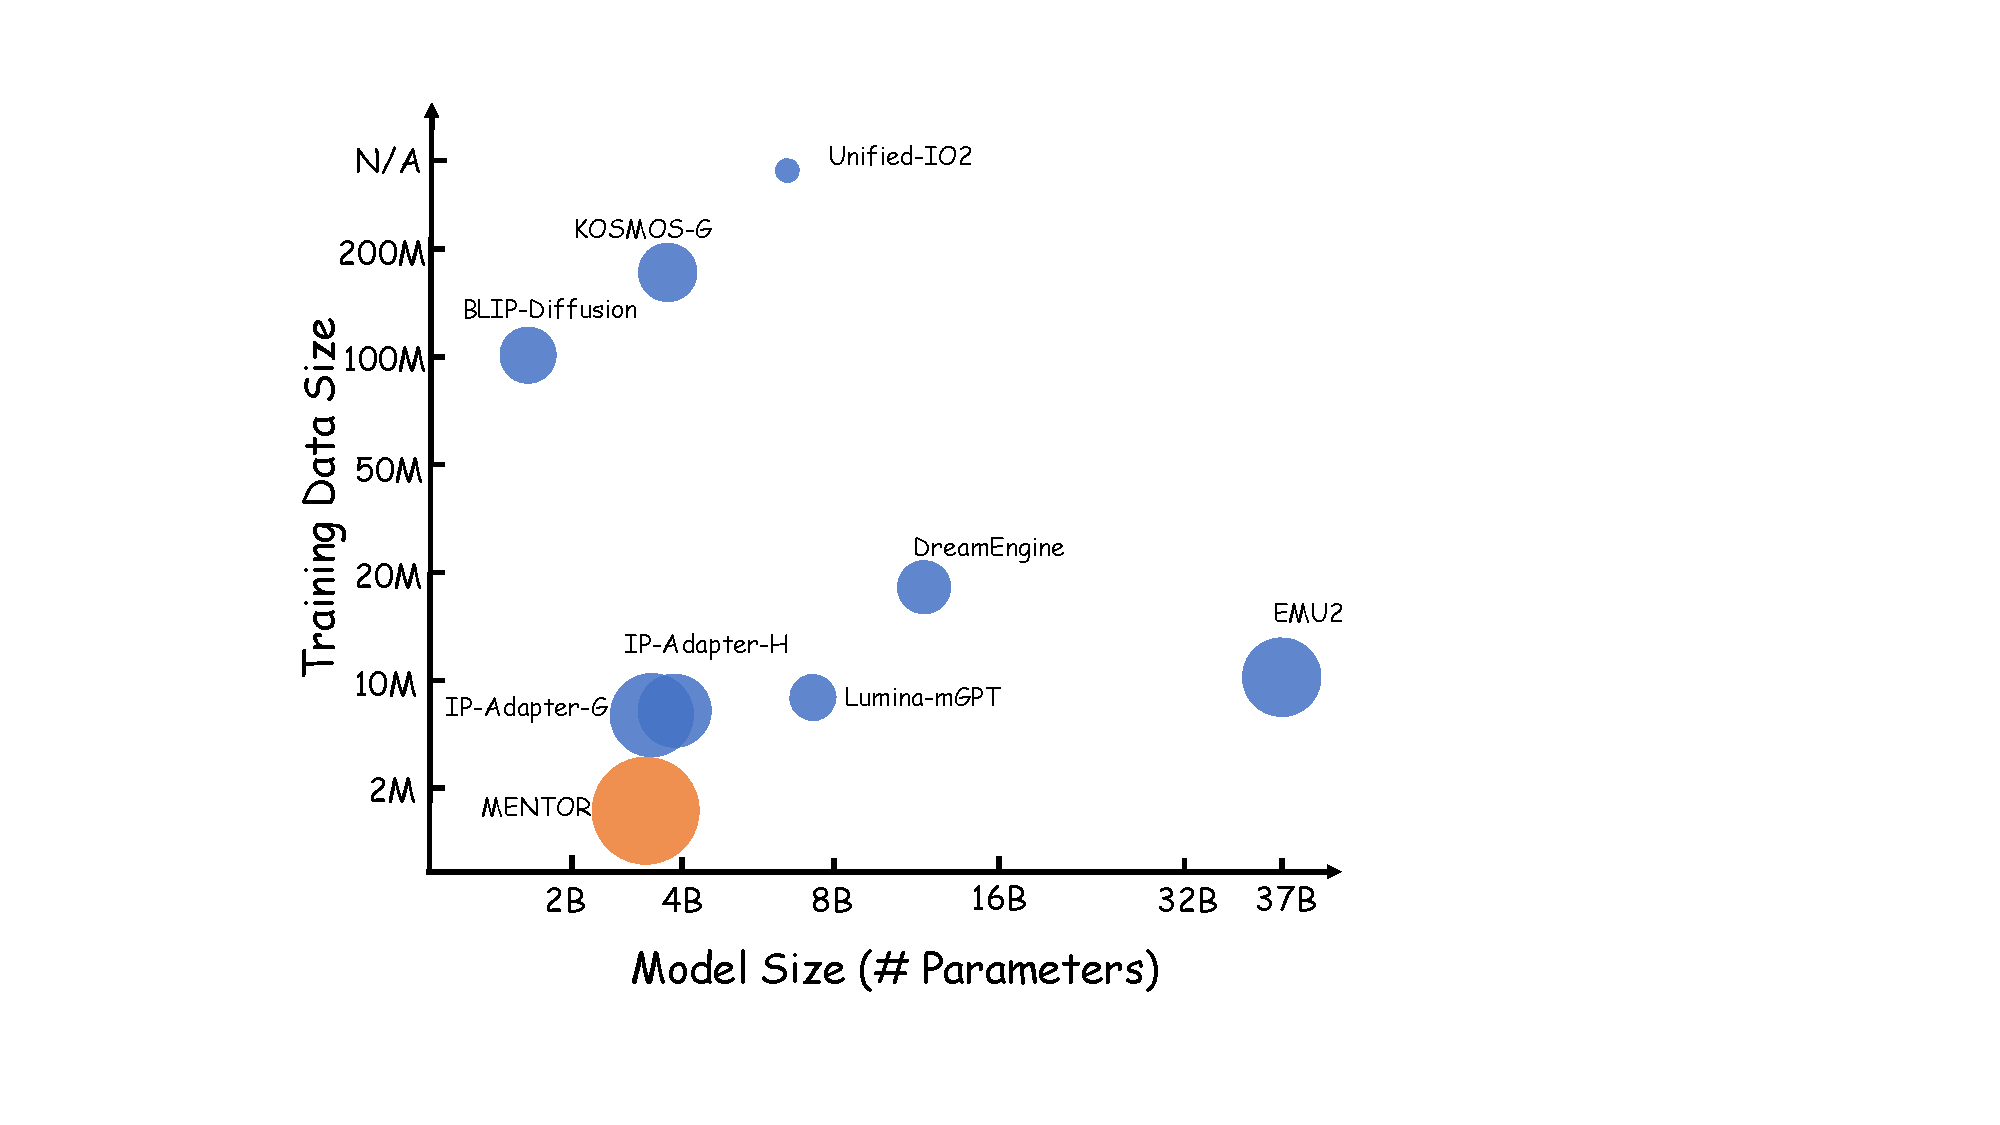
\includegraphics[width=\linewidth]{figures/Figure.pdf}
    % \caption{CP$\cdotp$PF score (circle size) of \model and other baselines on DreamBench++. Model in lower left achieves the best efficiency. }
    \caption{CP$\cdotp$PF score (circle size) of \textcolor[HTML]{ED8B50}{\textbf{\model}} and \textcolor[HTML]{5A76A9}{\textbf{other baselines}} on DreamBench++. Model in lower left achieves the best efficiency.}
    \label{fig:SnapKV}
    \vspace{-0.3cm}
\end{wrapfigure}



Recent progress in generative models has revolutionized text-to-image(T2I) generation~\citep{2020DDPM,ldm,SDXL}. However, real-world applications often require more than text-only prompts.
To achieve high-quality image generation, e.g., fine-grained control over generated images, the models need to seamlessly integrate multi-modal inputs, such as reference images with detailed instructions.
This poses significant challenges for existing diffusion models that are predominantly focused on T2I generation.
To address this, researchers have recently employed Large Multimodal Models (LMMs) to encode diverse inputs into unified embeddings compatible with diffusion models \citep{Kosmos-G, emu2}. While this approach aids in handling complex prompts for generation like interleaved image-text instructions \citep{emu2} or multimodal in-context learning \citep{Kosmos-G,2024SeedX}, several key limitations persist when scaling to complex multimodal control:

% Modern generative models have achieved remarkable success in image generation, with diffusion models leading the state-of-the-art performance in text-to-image generation~\citep{2020DDPM,ldm,SDXL}.
% Recent progress in generative models has revolutionized text-to-image generation with their remarkable capabilities\citep{2020DDPM,ldm,SDXL}.
% Along with their open-source communities, diffusion models dominate the field of visual generation up to today, particularly in text-to-image generation.
% However, real-world image generation applications often demand user interactions beyond simple text-only prompts. 
% To achieve high-quality image generation, e.g., fine-grained control over the generated images, the models need to seamlessly integrate multi-modal inputs, such as reference images, spatial layouts, stylistic exemplars, and detailed textual instructions.
% It poses significant challenges for existing diffusion models that are predominantly focused on text-to-image generation.

% Pervious methods have augmented diffusion models with auxiliary control mechanisms~\citep{controlnet, ye2023ip-adapter,ruiz2023dreamboothfinetuningtexttoimage}, enabling conditional generation guided by additional visual inputs. While effective in specific scenarios, these approaches often rely on task-specific adapters and specialized fine-tuning, which can limit their scalability and broader applicability. 
% Moreover, recent works integrate the large multimodal models (LMMs) with diffusion-based generators~\citep{Kosmos-G, emu2} to encode multimodal inputs into unified embeddings that are compatible with diffusion models, thereby supporting the multimodal conditional image generation.

% To address this challenge, early methods have augmented diffusion models with auxiliary control mechanisms.
% Approaches like ControlNet~\citep{controlnet} and DreamBooth~\citep{ye2023ip-adapter, ruiz2023dreamboothfinetuningtexttoimage} often rely on task-specific adapters and specialized fine-tuning, limiting their generalization ability.
% To address this challenge, more recently, researcher has leveraged Large Multimodal Models (LMMs) to encode diverse multimodal inputs into unified embeddings that are compatible with diffusion models~\citep{Kosmos-G, emu2}. This approach facilitates handling complex multimodal prompts, such as interleaved image-text instructions~\citep{emu2} or multimodal in-context learning~\citep{Kosmos-G,2024SeedX} for image generation.
% Nevertheless, despite their achievements, these methods still face several key limitations when scaled to complex multimodal control:





% To address this challenge, previous methods have augmented diffusion models with auxiliary control mechanisms, such as ControlNet~\citep{controlnet} and IP-Adapter~\citep{ye2023ip-adapter}~\citep{controlnet, ye2023ip-adapter,ruiz2023dreamboothfinetuningtexttoimage}, which often rely on task-specific adapters and specialized fine-tuning. 
% Moreover, others integrate Large Multimodal Models (LMMs) to encode diverse multimodal inputs into unified embeddings that are compatible with diffusion models~\citep{Kosmos-G, emu2}. These method aims to support more complex multimodal prompts, such as interleaved image-text instructions~\citep{emu2} or multimodal in-context learning~\citep{Kosmos-G,2024SeedX} for image generation.
% Despite promising in specific scenarios, these methods still face several key limitations when scaled to complex multimodal control:

% Despite these advances, existing methods still face significant challenges:
% \textbf{First}, the inherent randomness of diffusion processes complicates achieving precise and deterministic control, which is often necessary for tasks requiring high fidelity or accurate image reconstruction~\citep{wang2025imageeditingdiffusionmodels}. 
% \textbf{Second}, effectively balancing guidance of different modalities remains a persistent challenge. 
% Existing methods often struggle to integrate information harmoniously, sometimes over-emphasizing one modality while neglecting others~\citep{han2024emmatexttoimagediffusionmodel}. 
% For instance, methods like IP-Adapter~\citep{ye2023ip-adapter} and Lumina-mGPT~\citep{2024lumina}, which rely on text and image features as conditions, may predominantly be influenced by the image conditions.
% This imbalance can stem from the gap between modalities, which is further exacerbated by model architecture limitations~\citep{zhao2023mmicl,Dig2DIG,ye2023ip-adapter}, as well as suboptimal training paradigms~~\citep{Kosmos-G,han2024emmatexttoimagediffusionmodel}.
% \textbf{Third}, current diffusion-based methods~\citep{Kosmos-G,li2023blipdiffusionpretrainedsubjectrepresentation, emu2}, especially those incorporating auxiliary components for alignment(e.g., learned adapters~\citep{Kosmos-G}, regression heads~\citep{sun2023emu1,emu2}, specialized embeddings~\citep{seed-tokenizer}), typically necessitate extensive training on large-scale datasets~\citep{emu2,Kosmos-G,li2023blipdiffusionpretrainedsubjectrepresentation,2024SeedX}, incurring substantial computational costs.
% This is driven by the large parameter counts of individual components~\citep{emu2,Kosmos-G} (e.g., LLMs, diffusion backbones), auxiliary components, and the need for vast multimodal datasets.

\textbf{First,} the randomness of diffusion processes hinders precise, deterministic control, which is essential for high-fidelity tasks, like image reconstruction\citep{wang2025imageeditingdiffusionmodels}.
\textbf{Second,} balancing guidance from different modalities remains challenging. Existing methods frequently exhibit modality imbalance, often over-emphasizing one modality while neglecting others\citep{han2024emmatexttoimagediffusionmodel}. For instance, IP-Adapter \citep{ye2023ip-adapter} and Lumina-mGPT \citep{2024lumina}, conditioned on text and image features, may overly favor image inputs. This imbalance stems from modality gaps, architectural limitations \citep{zhao2023mmicl,Dig2DIG,ye2023ip-adapter}, or suboptimal training schemes \citep{Kosmos-G,han2024emmatexttoimagediffusionmodel}.
\textbf{Third,} many diffusion-based methods \citep{Kosmos-G, emu2}, particularly those with auxiliary alignment components (e.g., learned adapters \citep{Kosmos-G}, regression heads \citep{sun2023emu1,emu2}, specialized embeddings \citep{seed-tokenizer}), demand large-scale training \citep{emu2,Kosmos-G,li2023blipdiffusionpretrainedsubjectrepresentation,2024SeedX}, incurring substantial computational costs.
These challenges raise a critical question: \textit{Is there a more efficient and controllable paradigm for balancing complex multimodal conditions in image generation?}

% propose \textbf{\model}, a novel autoregressive (AR) framework for efficient \textbf{M}ultimodal g\textbf{E}neratio\textbf{N} \textbf{T}uning for aut\textbf{O}reg\textbf{R}essive multimodal image generation.
To address aforementioned limitations, we propose \textbf{\model}, a straightforward and efficient autoregressive (AR) framework for controllable multimodal image generation. Unlike diffusion models that rely on complex cross-attention layers for multimodal conditioning and demand extensive training resources \citep{2024SeedX,emu2,Kosmos-G,li2023blipdiffusionpretrainedsubjectrepresentation},  \model leverages a unified transformer architecture that directly aligns multimodal inputs with output image tokens. This design inherently simplifies architecture and training, reduces the need for auxiliary components for alignment, and significantly lowers training requirements.
Our framework employs a multimodal encoder to project multimodal inputs into a unified representation. An AR transformer decoder then generates image tokens deterministically, conditioned on this representation. To ensure effective and balanced modality integration, which is curial for multimodal image generation\citep{han2024emmatexttoimagediffusionmodel}, we adopt a two-stage training paradigm: (1) pretraining on image reconstruction and object segmentation to enable robust pixel-level and semantic alignment, followed by (2) multimodal instruction tuning with diverse tasks, such as image recovery and subject-driven generation, explicitly training the model to effectively leverage and balance varied multimodal inputs for coherent generation.

Notably, despite its simplicity and the use of suboptimal checkpoints, \model achieves state-of-the-art(SOTA) performance on the challenging DreamBench++ benchmark—using 10× less training data than leading baselines.
It outperforms resource-intensive baselines with powerful generators like SDXL \citep{SDXL} and SD3 \citep{2024SD3} by 30\% while dramatically reducing computational and data demands. 
Controlled experiments demonstrate the advantages of \model over diffusion-based methods in multimodal fidelity, training efficiency, and generation controllability.


 
% even with readily available multimodal encoders and modestly-sized autoregressive decoders, our method achieves state-of-the-art performance on the challenging DreamBench++ benchmark. It significantly surpasses resource-intensive baselines utilizing powerful generators like SDXL \citep{SDXL} and SD3 \citep{2024SD3} by 30\% while dramatically reducing computational and data demands. Extensive controlled experiments validate our AR approach's compelling advantages in multimodal fidelity, training efficiency, and generation controllability.

% In this paper, we propose a straightforward and efficient autoregressive (AR) framework explicitly designed for controllable multimodal image generation, directly addressing key limitations of prevalent diffusion-based approaches.
% including an AR generation model that suports multimodal conditions and a meticulously designed two-stage training paradigm.
% In contrast to diffusion-based methods that use cross-attention layers for multimodal conditioning and require extensive GPU resources for training, our approach directly aligns multimodal inputs with generated output tokens through unified autoregressive modeling in a simple transformer framework. It facilitates direct, token-level alignment between multimodal conditions and the generated image, providing a direct pathway for integrating diverse inputs.
% This inherent simplicity significantly reduces the reliance on task-specific adapters or extensive auxiliary components, leading to substantially lower training requirements.
% In contrast to diffusion-based methods that employ cross-attention layers for multimodal conditioning and typically necessitate extensive GPU resources for their training phases\citep{2024SeedX,emu2,Kosmos-G,li2023blipdiffusionpretrainedsubjectrepresentation}, our proposed method utilizes unified autoregressive modeling within a transformer architecture. This allows for the direct alignment of multimodal inputs with generated output tokens. 
% Such a direct pathway inherently simplifies the model architecture. 
% Consequently, it reduces the reliance on task-specific adapters or extensive auxiliary components for alignment and has significantly reduced training requirements.


% over diffusion-based counterparts.


% While pervious works like llamaGen~\citep{llamagen}, VILA-U~\citep{VILA-U}, EMU3~\citep{Emu3}, and the Janus-Series~\citep{Janus} have delved into autoregressive text-to-image generation, their capabilities for handling intricate multimodal conditions remain largely unexplored. 
% In contrast, our approach distinctively addresses multimodal conditional generation through the proposed AR framework and a carefully designed two-stage multimodal instruction tuning process. 
% By uniformly handling visual and textual inputs within a sequence-to-sequence modeling framework, our method paves the way towards more efficient, controllable, and robust multimodal generative systems.

% Through this implicit cross-modal alignment, achieved via token-level interactions, our approach substantially reduces the reliance on specialized modality adapters or extensive auxiliary components.
% This inherent simplicity translates directly into significantly reduced training requirements.
% Furthermore, to prevent the model from defaulting to a simple copy-paste function~\citep{han2024emmatexttoimagediffusionmodel} and overlooking textual conditions, our two-stage training process and diverse tasks ensure a nuanced understanding of visual input and a balanced integration of all modalities.


% Our framework utilizes a multimodal encoder to project heterogeneous inputs (visual and textual) into a unified latent space. An autoregressive transformer decoder then deterministically generates image tokens based on this unified representation. 
% To ensure robust understanding and balanced integration of diverse modalities—specifically preventing the model from defaulting to simple copy-paste function~\citep{han2024emmatexttoimagediffusionmodel} while ignoring textual instructions—we introduce a carefully designed two-stage training paradigm. In the first stage, the model is pretrained on image reconstruction and object segmentation tasks, fostering robust pixel-level and semantic-level alignment between the multimodal input and generated tokens. Subsequently, the second stage involves multimodal instruction tuning with diverse tasks, such as image recovery and subject-driven generation. This stage explicitly trains the model to leverage varied multimodal inputs effectively while balancing its focus across different modalities for coherent image generation.



% Specifically, our method employs a multimodal encoder to project heterogeneous inputs—visual and textual data—into a unified latent embedding space, creating a comprehensive multimodal representation. An autoregressive transformer-based decoder subsequently generates images based on this representation, producing deterministic outputs that accurately reflect the provided conditions.
% Building upon this architecture, we introduce a meticulously designed two-stage training paradigm. In the first stage, the model is pretrained on image reconstruction and object segmentation tasks, fostering robust pixel-level and semantic-level alignment and encouraging effective exploitation of visual information for image synthesis. 
% Subsequently, we perform the multimodal instruction tuning that incorporates additional training tasks, such as image recovery and subject-driven image generation. The second stage empowers the model to leverage varied multimodal inputs for image generation while explicitly balancing its focus across different modalities, enabling an efficient and robust fusion of multimodal information into coherent image outputs.

% Remarkably, even when employing readily available multimodal encoders and modestly-sized autoregressive decoders, our method achieves state-of-the-art performance on the challenging DreamBench++ benchmark. It surpasses the resource-intensive baselines, which utilize much more power generators like SDXL~\citep{SDXL} and SD3~\citep{2024SD3}, by xx\% while dramatically reducing computational and data resource demands. Through extensive controlled experiments, we directly compare our AR approach with diffusion-based counterparts and demonstrate compelling advantages in multimodal fidelity, training efficiency, and generation controllability.

% our method surpasses other baselines and achieves state-of-the-art performance on the challenging DreamBench++ benchmark by xx\%, while dramatically reducing computational and data resource demands. We also conduct extensive controlled experiments comparing our autoregressive approach directly with diffusion-based paradigms. 
% Our findings demonstrate that autoregressive models offer significant advantages in multimodal fidelity, generation controllability, and consistency.


% Our contributions are summarized as follows:
% \begin{itemize}[left=2pt]
% \item We propose a novel autoregressive framework for efficient multimodal image generation tuning, demonstrating state-of-the-art performance with substantially reduced training resources.
% \item We introduce a two-stage training strategy to align multimodal embeddings effectively, enabling balanced multimodal attention and precise conditional adherence.
% \item Extensive experiments validate the superior efficiency and multimodal capabilities of our AR framework, highlighting its potential as a scalable alternative to existing diffusion-based methods.
% \end{itemize}
Overall, our contributions are as follows: (1) A novel autoregressive framework for efficient multimodal generation, achieving, achieving SOTA performance; (2) A two-stage training strategy for multimodal-conditioned tuning, enabling robust alignment and balanced modality integration with significantly reduced training cost; (3) Extensive experiments demonstrating the superior efficiency, controllability, and fidelity of \model as a compelling alternative to diffusion-based methods.



% Our contributions are:
% \begin{itemize}[left=2pt]
%     % \setlength\itemsep{0.1em}
%     \item A novel autoregressive framework for efficient and controllable multimodal  generation, achieving state-of-the-art performance with substantially reduced training resources.
%     \item A two-stage training strategy to ensure robust multimodal alignment and balanced integration of diverse modalities for controllable multimodal image generation.
%     \item Extensive experiments validating the superior efficiency, controllability and multimodal fidelity of \model, highlighting its potential as a scalable alternative to the diffusion-based methods.
% \end{itemize}



% The proposed model integrates a multimodal encoder with a unified transformer decoder. The multimodal encoder is responsible for processing and fusing multimodal inputs into a coherent conditioning representation. It converts each input into combined latent token sequence for generation. This encoded sequence of tokens serves as deterministic context for the decoder. The unified transformer decoder then autoregressively generates the output image token-by-token. 

% Thanks to this design, our model can seamlessly integrate information from multimodal conditions and synthesize a new image that precisely reflects all these inputs, leading to three key advantages:

% \begin{itemize} 
% \item \textbf{Deterministic Control.} The absence of stochastic sampling enables consistent and interpretable outputs, supporting precise image reconstruction and fine-grained editing.
% \item \textbf{Multimodal Instruction Following.} Both language and vision are treated uniformly as token sequences, enabling seamless cross-modal attention and better instruction following for image generation. 
% \item \textbf{Training Efficiency.} Unified autoregressive modeling facilitates the direct alignment of multimodal inputs with output sequences. This implicit shortcut reduces reliance on modality-specific alignment modules, and also significantly lowers training costs.
% \end{itemize}



% Our AR model achieves state-of-the-art performance on the DreamBench++ benchmark, outperforming prior diffusion-based methods. Notably, our approach attains this strong performance with far fewer resources. In fact, even with sub-optimal large multimodal modules as the encoder and a relatively low-capacity image decoder, our AR framework matches surpasses other baselines. This highlights the training efficiency and effectiveness of our proposed paradigm – by treating generation as a discrete sequence prediction, we sidestep the need for large training data and lengthy training schedules, yet still capture the complex relationships between multimodal inputs and outputs.

% Furthermore, we conduct extensive controlled experiments to directly compare the AR and diffusion paradigms in multimodal conditional generation scenarios
% Our findings reveal that autoregressive models offer a promising and underexplored alternative for conditional image generation, particularly in multimodal settings requiring fine-grained control and interpretability. By unifying visual and text inputs in a sequence-to-sequence formulation, our approach paves the way toward more controllable and efficient generative systems.



% efficiency : model size training data
